\documentclass{article}

\usepackage{newspaper}
\date{\today}
\currentvolume{2019}
\currentissue{1}
\usepackage{times}
\usepackage{graphicx}
\usepackage{multicols}
\usepackage[czech]{babel}
\usepackage[utf8]{inputenc}
\usepackage{lettrine}

\usepackage{picinpar}
%uasage of picinpar:
%\begin{window}[1,l,\includegraphics{},caption]xxxxx\end{window}

\widowpenalty=10000
\clubpenalty=10000

%%%%%%%%%  Front matter   %%%%%%%%%%

\makeatletter
 \def\ps@myinfo{
 \def\@oddfoot{
	\begin{center}
             {\setlength\fboxsep{3mm}\raisebox{12pt}{\framebox[\textwidth]{\parbox[c]{\textwidth}{
                 \begin{center}\small Tršický Zpravodaj, zpravodaj obce Tršice; periodický tisk územního samosprávného celku; vydává Obec Tršice, Tršice 50, Tršice 783 57, IČ: 00299588; registrace u MK ČR E 12519 
                 \end{center}}}}}\hfill
         \end{center}}
 \def\@evenfoot{
	\begin{center}
             {\setlength\fboxsep{3mm}\raisebox{12pt}{\framebox[\textwidth]{\parbox[c]{\textwidth}{
                 \begin{center}\small Tršický Zpravodaj, zpravodaj obce Tršice; periodický tisk územního samosprávného celku; vydává Obec Tršice, Tršice 50, Tršice 783 57, IČ: 00299588; registrace u MK ČR E 12519 
                 \end{center}}}}}\hfill
         \end{center}}
}
\makeatother

\begin{document}
\maketitle

\centerline{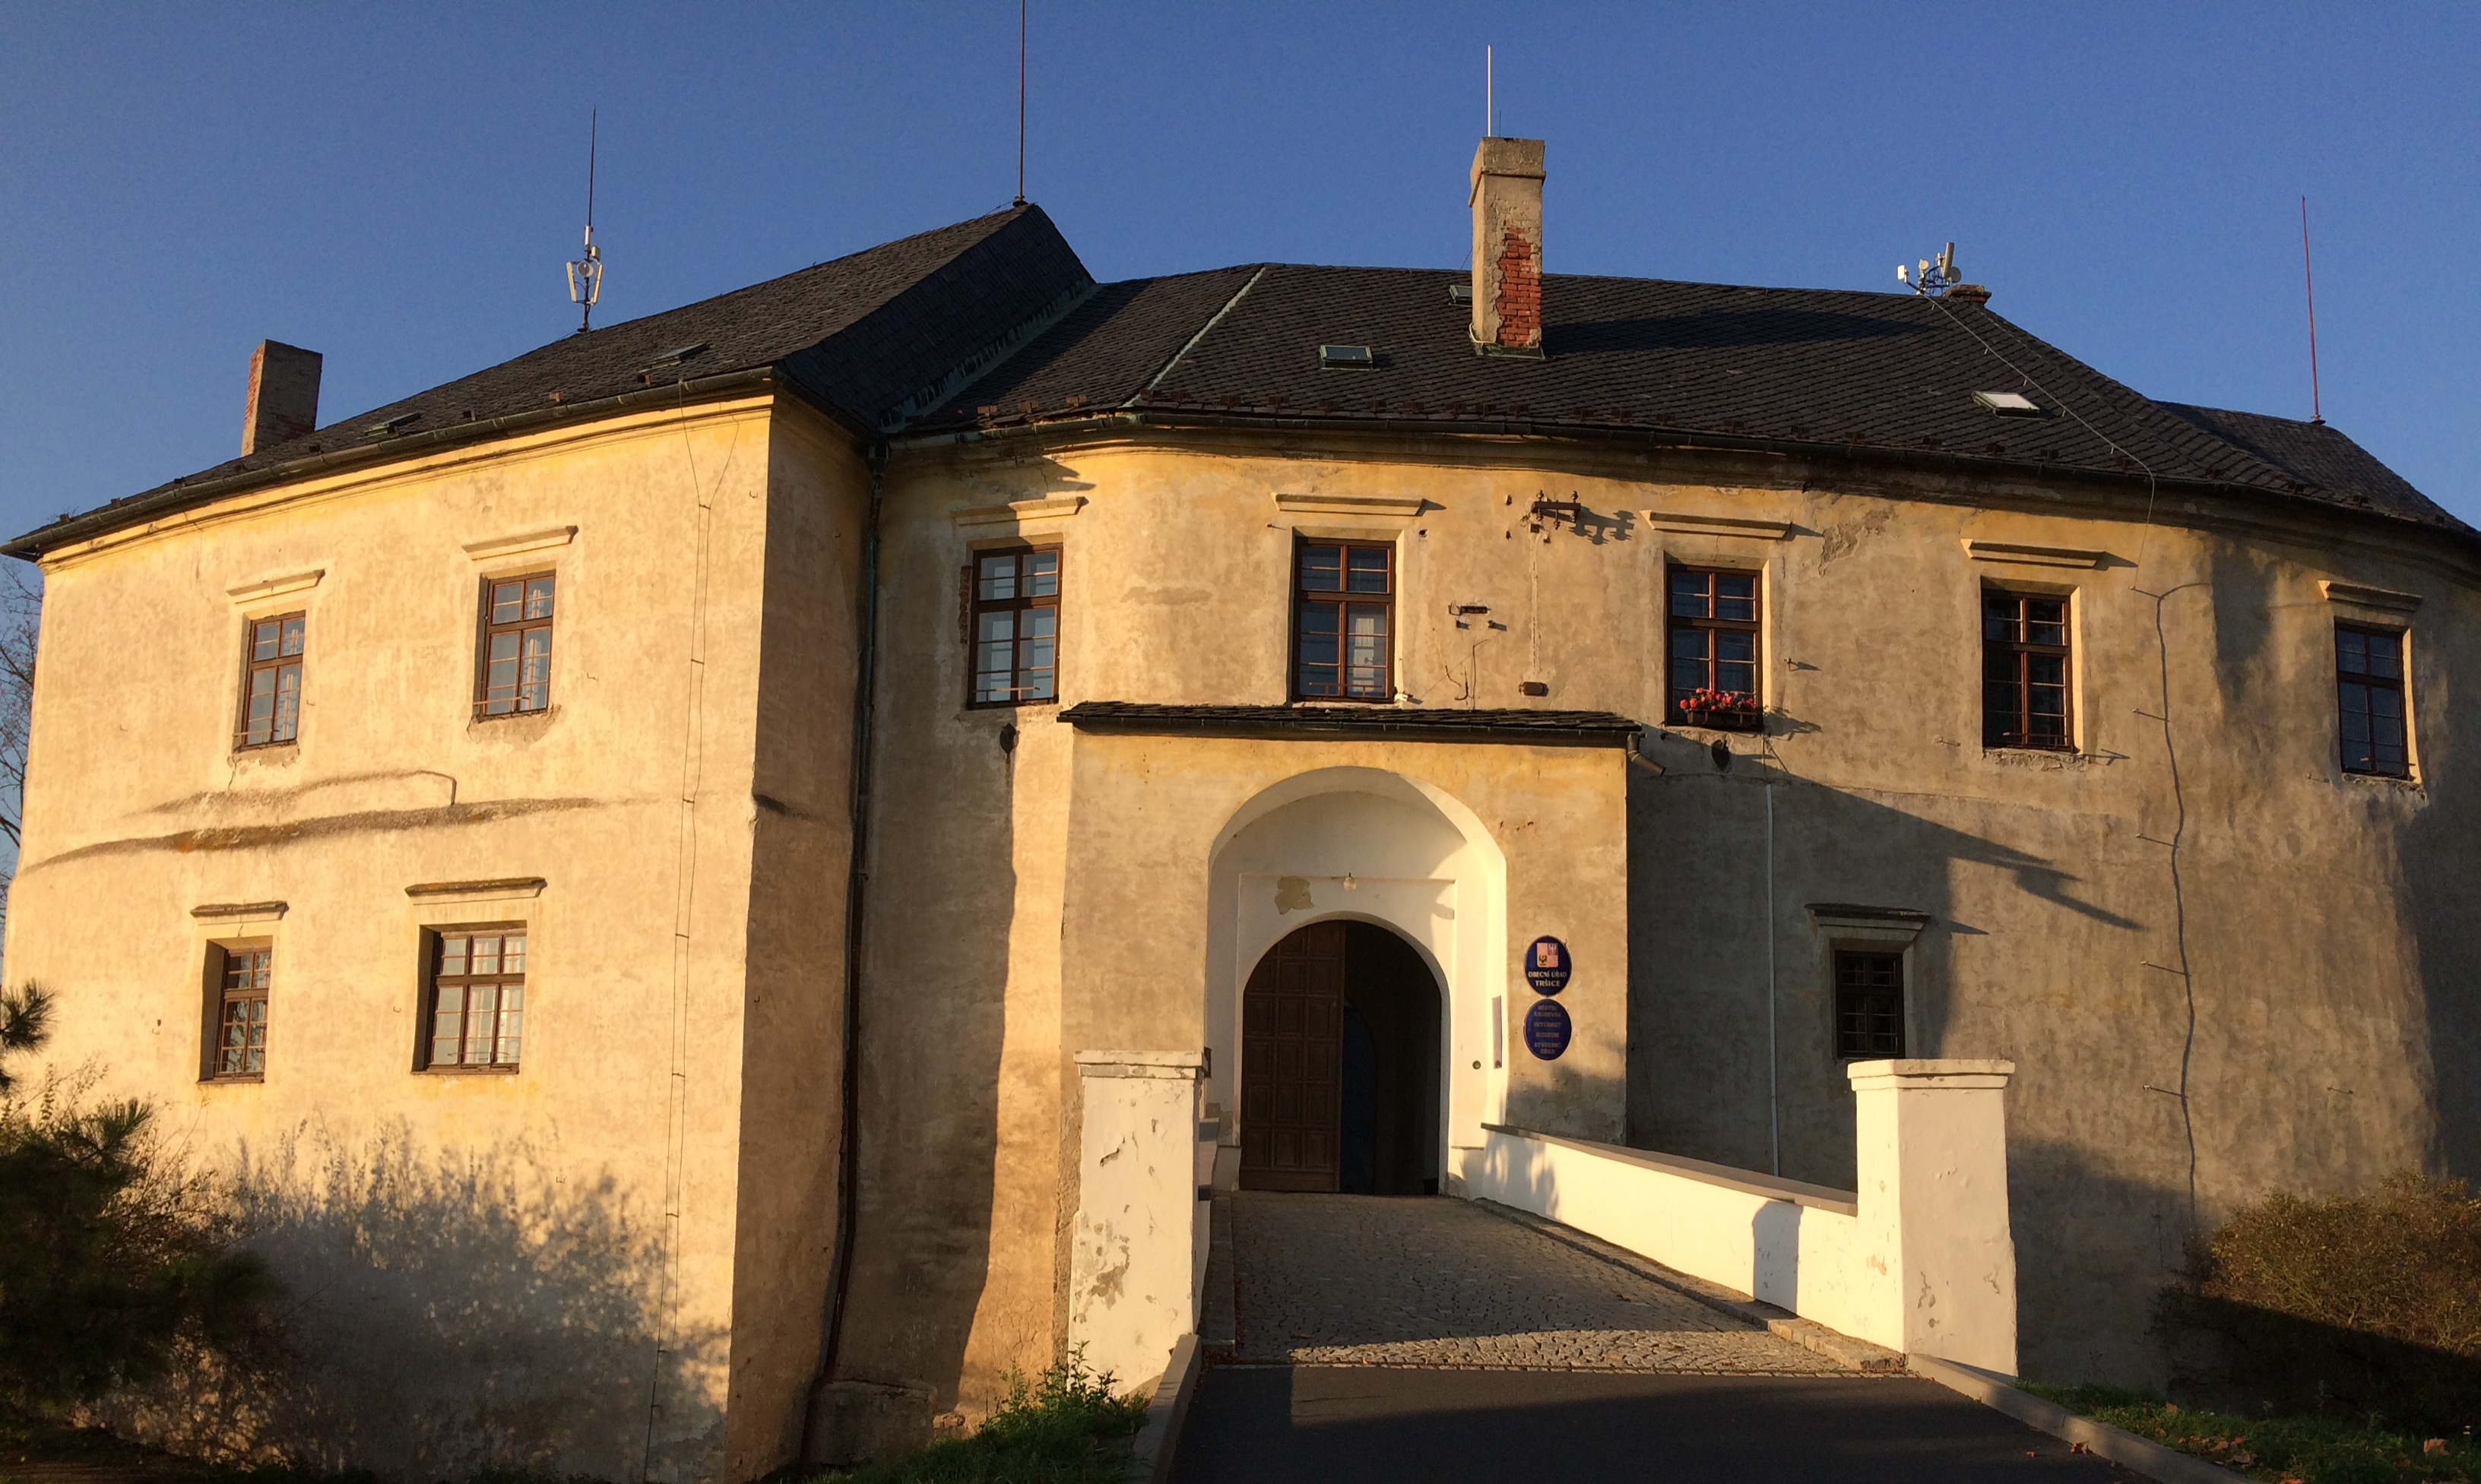
\includegraphics[width=0.90\textwidth]{zamek-trsice.jpg}}

\byline{\it\Huge Slovo starosty}{Pavel Kováček}
\begin{multicols}{3}{

\lettrine{V}{ážení} spoluobčané, jsem velice potěšen, že Vás mohu prostřednictvím prvního vydání obnoveného Tršického zpravodaje, ze kterého jste se mohli dozvědět něco o dění v naší obci naposledy v roce 2017, informovat o průběhu činností a plánů, které jsme od ustavující schůze zastupitelstva, konané 31.10.2018, učinili a společnými silami naplánovali.

Zároveň bych Vám chtěl za všechny zvolené zastupitele poděkovat za Vaši důvěru, kterou jste do nás vložili, a jsem opravdu přesvědčen, že se nám společnými silami podaří v naší obci i v přilehlých částech, vytvořit podmínky pro spokojený život všech občanů.

Prostřednictvím Tršického zpravodaje Vás informujeme až nyní, jelikož informace, které jsme obdrželi od bývalého vedení obce, byly velice stručné a nebylo možné Vás dostatečně a průběžně informovat o tom, jak budeme ve vedení obce dál pokračovat. Po mém zvolení do funkce starosty obce bylo nutné převzít úřad od předchozí starostky a zjistit stávající stav dosavadních činností obecního úřadu, tak aby převzetí nenarušilo plynulý chod, a aby byl i nadále obecní úřad přístupný potřebám občanů. Samotné předání úřadu a k tomu navazujících informací o tom, co je nutné v následujících dnech, týdnech a měsících provést, bylo velmi rychlé a trvalo asi hodinu. Nebylo tedy úplně možné plynule navázat na chod obce a rozběhnuté projekty. Společně s místostarostou, s některými kolegy ze zastupitelstva a se členy výborů jsme k problematice přistoupili tak, abychom zabezpečili plynulý chod úřadu, avšak zároveň i s celkovými kontrolami a revizemi všech středisek, aby nedošlo k žádným škodám na majetku obce, kde mezi hlavní patřilo účetnictví a finanční správa obce. O té Vás v dalším článku bude informovat finanční výbor.

\begin{window}[2,r,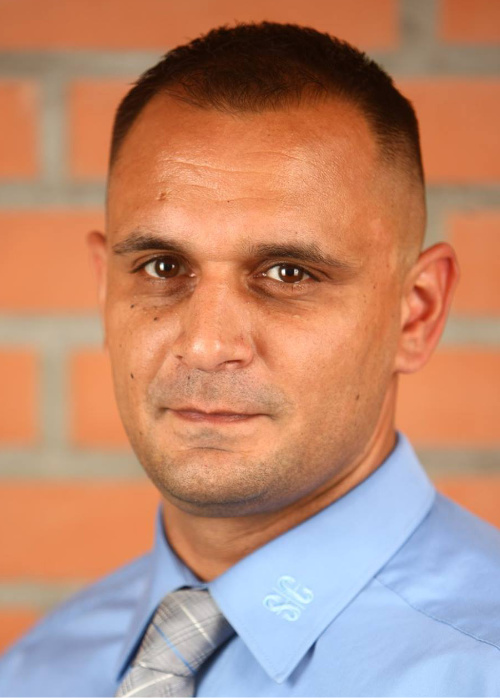
\includegraphics[width=1.5in]{starosta.jpg},\centerline{\emph{Starosta obce}}] S převzetím funkce souviselo i převzetí obsluhy čistírny odpadních vod. Zde nastala závažná komplikace, neboť v den ustavujícího zasedání zastupitelstva podali zaměstnanci obecního úřadu, odpovědní za provoz čístírny odpadních vod, výpověď, která byla bývalým vedením akceptována dohodou bez obvyklé dvouměsíční výpovědní lhůty. K předání čistírny odpadních vod (ČOV) tedy nedošlo, ani ze strany bývalé starostky, ani ze strany předchozího správce. Tato skutečnost nám způsobila velké komplikace, už jen s ohledem na skutečnost, že k obsluze ČOV pochopitelně nikdo z nového vedení obce není kompetentní. Na ČOV se nacházejí různé technologie, například živé kultury k rozkladu kalu, a kdyby se nám nepodařilo je včas stabilizovat, došlo by k velkým finančním ztrátám. Magistrát města Olomouce – odbor životního prostředí tedy hned první den mého působení v úřadu, 1. 11. 2018, požadoval neprodleně nahlásit, kdo bude dělat odborný dozor nad ČOV, bez kterého je dle zákona o vodách a kanalizacích nepřípustné provozovat čištění odpadních vod a dodávat pitnou vodu. Následovalo zajištění prioritních úkonů vzhledem k provozu ČOV, abychom se nedostali do situace, kdy by mohlo dojít k finančním nebo materiálním škodám, od kterých jsme bohužel nebyli daleko. Odborníci, se kterými jsme konzultovali naše možnosti, nám sdělili, že s takovým případem předání se ještě nesetkali a že ohrožením živých kultur byla obec vystavena možným vysokým finančním nákladům. Ve spolupráci s pracovníkem ČOV Doloplazy, kterému děkujeme za vstřícný přístup a který nám zpočátku nesmírně pomohl, jsme získali důležitou počáteční kontrolu nad provozem ČOV. Musím konstatovat, že i pro pracovníky obecní čety to bylo velice náročné. Obsluhovat ČOV a zároveň provádět běžnou práci týkající se provozu obce, je ve třech lidech takřka nadlidský výkon. Nicméně podařilo se a my jsme měli v tu chvíli prostor pro zajištění odborného dozoru. Po měsíci konzultací a vyjednání byly podepsány smlouvy s externí firmou Aqua-Styl, která nám zajišťuje odborný dozor a zabezpečuje všechna hlášení, která se musí na začátku roku posílat na příslušné úřady. Po třech měsících můžu s malou nadsázkou říct, že po všech těch konzultacích, kterých jsem se zúčastnil mi připadá, že jsem se stal téměř odborníkem na obsluhu ČOV. Znamená to tedy, že nyní máme ČOV plně pod naší kontrolou a stálou obsluhu zajišťují zaměstnanci obecního úřadu.
\end{window}

Rád bych Vás také informoval o vyúčtování vodného a stočného za rok 2018. S ohledem na to, že databáze vedená předchozím správcem byla nedostatečná, a v této chvíli nemáme k dispozici dostatek dat potřebných pro řádné stanovení ceny (problémem jsou zejména chybějící nebo neplatné smlouvy, neregistrovaná čísla vodoměrů a odběrných míst), není snadné spočítat ceny za odběr vody a stočné. Jsme nuceni provést kompletní kontrolu všech odběrných míst osobně a zaevidovat všechny potřebné údaje. Jistě si dovedete představit, vážení občané, že úkol to není snadný. Abychom v budoucnu předešli zmatkům a finančním ztrátám, které v minulosti vznikaly, je nutné vytvořit přehlednou databázi všech odběratelů spojenou s vyhotovením nových smluv, které budou obsahovat všechny potřebné údaje a informace, jak pro odběratele, tak i pro dodavatele. Chceme totiž, aby bylo ze smlouvy na první pohled zřejmé, z čeho je výpočet prováděn a kolik má odběratel platit. Z dat které jsme v této chvíli nasbírali vyplývá, že proběhne další kolo zjišťování potřebných informací. S ohledem na množství odběratelů a množství chybějících dat, předpokládáme dokončení vyúčtování v průběhu března tohoto roku. Děkuji odběratelům za pochopení a součinnost při kontrolách prováděných pověřenými pracovníky.

Za uplynulé tři měsíce mohu říct, že se nám také podařilo navázat na projekty, které jsou rozpracovány z předchozího období. Mezi hlavní patří výstavba nové hasičské zbrojnice, kde po provedení nutných úkonů k přípravě můžeme přistoupit k další etapě projektu, a tím je zajištění služeb pro výběrové řízení, s ohledem na splnění požadavků pro realizaci. Demolici stávající hasičské zbrojnice předpokládáme v druhé polovině tohoto roku a čeká nás tedy nelehký úkol zajistit prostory pro jednotku požární ochrany obce Tršice (JPO) . Společně s nimi ztratí své prostory i pracovníci z obecní čety, kteří mají v prostorách plánované demolice svojí dílnu a sociální zázemí. Minulé zastupitelstvo toto neřešilo, nebude to lehký úkol, avšak jsem přesvědčen, že najdeme vhodné prostory pro náhradní zázemí všech těchto složek. Náklady na vybudování nové hasičské zbrojnice, které přesahují 14 mil. Kč, bude financovat obec z vlastního rozpočtu, ve kterém jsou tyto investice zahrnuty ve dvou etapách pro rok 2019 a 2020. Tyto budou následně proplaceny z dotace, která pokrývá 90 \% celkových uznatelných nákladů. Bylo nutné tyto výdaje dobře plánovat s ohledem na to, abychom již více nezhoršovali finanční situaci obce, kde zadluženost nyní dosahuje 79 \% plánovaných příjmů obecního rozpočtu.

I tak je ale nutné konstatovat, že přes veškeré plány se, můžeme dostat do situace, kde by nebylo možné ufinancovat jak výstavbu, tak i chod obce, už s ohledem na to, že od voleb do zastupitelstva je finanční stav obce velmi špatný. Důvodem bylo mimo jiné to, že v předchozím roce se uskutečnilo několik projektů, které nebyly plánovány v rozpočtu obce pro daný rok, nebylo tedy pro ně připraveno financování. Bylo tedy úkolem nového zastupitelstva přijmout rozpočtové opatření k legalizaci těchto akcí a část plateb ve výši 2 mil. Kč přesunout do rozpočtu roku 2019. Z těchto důvodů je pro nás nutné vyhotovit plán finančních rezerv, ze kterých v případě nutnosti budeme moci zabezpečit financování vzniklých komplikací.

Závěrem mého úvodního slova tohoto zpravodaje bych Vám chtěl poděkovat za určitou schovívavost v případech, kdy nelze Vaše záležitosti – a je jich opravdu mnoho – vyřešit hned a chtěl bych Vás touto cestou ubezpečit, že ve spolupráci s pracovníky obecního úřadu, se zastupiteli a také se členy výborů, řešíme tyto úkoly v nejbližším možném termínu.

V roce 2019 Vám přeji hodně zdraví a štěstí a mnoho osobních i pracovních úspěchů a jsem přesvědčen, že nejen vydáním prvního čísla zpravodaje obnovíme dobré vztahy mezi obecním úřadem a občany.

\emph{Váš Pavel Kováček, starosta obce Tršice.}
}\end{multicols}

\closearticle

\begin{multicols}{2}{
\byline{\sc\Large Zpráva finančního výboru}{Marek Závodník}

\lettrine{V}{ážení} spoluobčané. Dovolím si využít historicky první příležitosti seznámit Vás s děním v Tršicích a  přidružených obcích z pohledu peněžního, očima finančního výboru zastupitelstva obce Tršice. A to po dlouhých letech a několika volebních obdobích, kdy jsem alespoň já osobně měl neodbytný pocit, že obecní peněžní toky zůstávaly občanům ukryty za strohými čísly účetních výkazů a paragrafů, které se tu a tam objevily na úřední desce. Parta ,,Našim dětem'' to ale vidí jinak a budeme se proto snažit tento neutěšený stav postupně napravovat a nechat kohokoliv, kdo bude mít zájem, nahlížet \uv{pod pokličku}.

Finanční výbor je zřizován povinně ze zákona a jeho hlavním úkolem je kontrola hospodaření s majetkem obce, tedy nás všech. Finanční výbor dohlíží na to, zda jsou peníze a ostatní majetek obce užívány v souladu se zákonem, se schváleným rozpočtem obce a hlavně efektivně, tedy z pozice řádného hospodáře. Členy finančního výboru byli na ustanovující schůzi zastupitelstva obce zvoleni Jiří Rozsíval starší, Pavel Šimeček a Marek Závodník. Jiří je absolventem Vysoké školy chemicko-technologické v Praze, má bohaté zkušenosti ze soukromého podnikání, Pavel je absolventem Vysoké školy ekonomické v Praze a profesionální auditor, já jsem vystudoval na Ekonomické fakultě Masarykovy univerzity v Brně a profesně zodpovídám za správu majetku aktuálně osmi akciových společností. Jsem opravdu rád, že mi bylo umožněno pracovat v takovém týmu schopných lidí, kteří rozumí tomu, co dělají a byli ochotni věnovat spoustu svého volného času veřejnému zájmu. Ne vždy je tato práce na první pohled viditelná.

Je mi líto, že jsme neměli možnost Vás informovat o tom, co se děje s obecními penězi už dříve, ale má to své důvody. Tím prvním bylo zcela nedostatečné předání obecní agendy bývalým vedením obce. Co v jiných obcích trvá dny až týdny, se v Tršicích událo za necelou hodinu. K dispozici tak stále nemáme seznam rozpracovaných akcí, neznáme současné ani budoucí závazky, marně dohledáváme příslušné dokumentace a smluvní vztahy. Co jsme ale obdrželi, je neutěšený stav obecních financí, kdy na peněžních účtech nebyl dostatek prostředků ani na běžný provoz obce a hrazení faktur (úhradu nákladů za rekonstrukci kanalizace v Chaloupkách jsme z důvodu nedostatku peněz museli odložit až na letošní rok). Jak jsme poměrně brzy zjistili, stalo se tak mimo jiné z důvodu překotného a nesystémového financování rekonstrukce komunikací v předvolebních měsících (v celkové výši cca 7,5 milionů Kč) a urychlené a nedokončené výstavby dětských hřišť (celkem 1,5 milionu Kč, z toho jen nedokončené dětské hřiště v Tršicích spolklo 800 tisíc Kč). Velká část těchto peněz byla utracena v rozporu se schváleným rozpočtem obce na rok 2018 (tedy v nesouladu se zákonem), a byla převedena z prostředků původně určených na rekonstrukci obecních bytů, výdajů na sport a údržbu veřejné zeleně. Tyto nestandardní finanční operace muselo zpětně napravit nové zastupitelstvo obce rozpočtovým opatřením č.4-2018, kdy nám nezbylo nic jiného, než tyto transakce zpětně schválit a uvést je do souladu s rozpočtem. Získat tyto peníze tam, kam původně patřily, už se nám nepodaří, protože byly utraceny.

V listopadu loňského roku došlo také ke skokovému nárůstu mzdových nákladů z průměrných 544 tis. Kč na 1 mil. Kč, na čemž se podílela nejen zákonná odměna odstupující starostky, ale i vyplacení mimořádných odměn některým pracovníkům. A jednalo se o tak kvalitní a potřebné pracovníky, že ukončení jejich pracovního poměru dohodou bylo přijato ještě v den podání, shodou okolností poslední den funkčního období bývalého vedení obce. Dlužno dodat, že jejich náhlý odchod způsobil obci značné provozní problémy.

Z důvodu absence jakéhokoliv kontrolního mechanismu, kdy veškeré důležité informace byly drženy jedinou osobou bez širší diskuze alespoň v rámci zastupitelstva, jsme byli nuceni vyplýtvat spoustu času na to, abychom zjistili, jak vedení obce vlastně fungovalo. Jsme teprve v půli cesty, ale už dnes víme, že musíme řešit nestandardní nákupy externích služeb, absenci smluv, realizaci investičních akcí bez řádné odborné přípravy, efektivity a důslednosti, což už bohužel nese první neblahé důsledky pro nás všechny: Pochybné závazky obce, které budeme dále řešit (např. obdržená faktura od dodavatele za čištění obecní kanalizace za téměř půl milionu korun bez relevantních podkladů, a to na základě objednávky bez stanovené ceny a rozsahu prací), nutnost vyplacení bezdůvodného obohacení obce Tršice vůči Úřadu pro zastupování státu ve věcech majetkových ve výši 81 tis. Kč za neuplatnění nároku na zápis vlastnického práva k pozemkům na Zákřově, nebo obdržená pokuta ve výši 40 tis. Kč za nesplnění smluvní povinnosti uzavřít smlouvu o zřízení věcného břemene v rámci výstavby ČOV. Budeme pátrat po příčinách vzniku těchto nákladů a vymáhat je po vinících.

V neposlední řadě s sebou, jako pověstnou kouli na noze, táhneme břemeno vysokého dluhu: Obec Tršice patří mezi 7\% nejzadluženějších měst a obcí v celé České republice. Aktuální výše nesplaceného dluhu je téměř 29 milionů Kč. Pro porovnání: Většina obcí mikroregionu Bystřička má obecní dluh nulový. Nejvyšší dluh má aktuálně obec Přáslavice, a to pětkrát menší než ten náš. Výmluvně to vypovídá o způsobu nakládání s obecními penězi, protože i naši sousedé budovali ČOV, vodovod nebo stavěli nákladné cesty.

Velkým tématem jsou pro nás dotace: Prostředky přerozdělované z veřejných zdrojů (od Kraje, Evropské unie, státu apod.). Finanční výbor bude prosazovat využívání dostupných dotačních titulů, ale v každém případě budeme předcházet zbrklým a neodborně připraveným akcím, které podle náhledu do dostupných materiálů budí dojem, že sloužily spíše k podpoře profesionálních agentur, které tyto dotace zprostředkovávají a velmi slušně na nich vydělávají právě na úkor obcí. Budeme Vás průběžně informovat o skutečných nákladech již dokončených, probíhajících i plánovaných akcí spolufinancovaných z dotačních titulů. V mnoha případech se totiž ukazuje, že pro obec by bylo levnější danou investici zrealizovat z vlastních zdrojů, než zaplatit vysoké zprostředkovatelské poplatky a spoluúčast na neefektivně nastavené dotace.

Naším nejdůležitějším cílem je stabilizovat, očistit a zprůhlednit finanční stav obce. Základním viditelným výsledkem je schválená podoba rozpočtu obce na rok 2019 a střednědobý finanční výhled, za jehož přípravu musím poděkovat hlavně Pavlovi Šimečkovi a paní Janě Ulicové, která má na starosti vedení účetnictví obce. I se stávající výší dluhu (chtě nechtě musíme splatit 228 tisíc Kč měsíčně) se nám podařilo navýšit množství peněz určených pro Základní školu a Mateřskou školu v Tršicích (2,5 milionu Kč), po dlouhé době získá finanční podporu obce také SRPŠ. Připraveny máme prostředky na postupnou rozsáhlou rekonstrukci veřejného osvětlení ve všech našich obcích (řádově miliony korun každý následující rok), vybudování nové hasičské zbrojnice, opravy cest a chodníků, vyšší podporu místních spolků. Investovat budeme také do zvelebení a rozšíření hřbitova, kde plánujeme vybudování parkoviště a chodníků. Finanční výbor navrhne zastupitelstvu obce úpravu výše nájmu za pořádání kulturních akcí na obecním sále na symbolickou 1,- Kč pro místní spolky.

Prosím, pokud budete mít dotaz, připomínku, dejte nám vědět. Rádi se jí budeme věnovat, jak jen nejlépe budeme umět. Přejeme si, aby se obecní úřad v Tršicích stal místem, kam budou občané chodit s chutí a úsměvem.

}\end{multicols}

\begin{multicols}{2}{}\end{multicols}

\closearticle

\begin{multicols}{3}{

\byline{\it\Huge Tršický zpravodaj}{Martin Polák}

\lettrine{J}{ak} vidíte, milí čtenáři, po nějaké době opět ožívá Tršický zpravodaj. V jeho vydávání nastanou některé změny, se kterými bych vás rád seznámil.

Především chceme zprovoznit internetovou verzi Tršického zpravodaje. V dnešní době má už většina lidí přístup k internetu, ať už z počítače nebo z mobilního telefonu. V internetové verzi by vycházely články průběžně, tak jak vznikají, a každý by měl možnost si je kdykoliv přečíst. Několikrát do roka (podle množství článků) by potom vyšla také tištěná verze, která by byla pro zájemce k dispozici na obecním úřadě, v obchodech a podobně. Tím bychom ušetřili náklady na tisk a také zbytečně neplýtvali papírem. Počet tištěných kusů postupně upravíme podle zájmu.

Obsahově chceme samozřejmě přinášet články o dění v naší obci, škole, spolcích. Také o historii obce a dění v minulosti. Ale přivítáme i články, které s naší obcí přímo nesouvisí. Třeba o zajímavém koníčku, zálibě, prostě o čemkoli, co by mohlo být pro čtenáře zajímavé. Vítáme každého zájemce o spolupráci. Pokud budete mít zájem, dejte vědět na obecní úřad nebo můžete kontaktovat přímo mě na emailové adrese \emph{martin@nigol.cz}.

Myslím, že existence našeho Zpravodaje je důležitou součástí informovanosti lidí o dění v obci. Máme tu formální zdroje informací, jako jsou internetové stránky obce nebo úřední vývěska, a potom potřebujeme také méně formální zdroj informací a třeba i zábavy – například Tršický zpravodaj. Pokusme se jej udělat co nejzajímavější.

}\end{multicols}

\closearticle

\begin{multicols}{3}{

\byline{\sc\Large Informační technologie v naší obci}{Martin Polák}

\lettrine{F}{ungující} počítačové vybavení je v dnešní době nezbytným předpokladem pro výkon obecní samosprávy. Obec je ze zákona povinna vést některé agendy a též je povinna komunikovat s úřady a dalšími subjekty i elektronicky. Také je vhodné, pokud je v dnešní době obec schopna komunikovat pomocí moderních kanálů i s občany. Bez fungujícího technického zázemí je to problematické.

Rozdělme si problematiku na dvě oblasti. První je vnitřní vybavení, které je třeba pro samotný chod úřadu – zejména počítače zaměstnanců + potřebné vybavení, za druhé pak vybavení pro vnější prezentaci obce – především internetové (webové) stránky obce, emailové adresy a podobně.

Začněme tedy vybavením, které je nezbytné pro vnitřní fungování úřadu. Všichni zaměstanci, pracující v kanceláři, mají k dispozici počítač s potřebným programovým vybavením. To se na jednotlivých počítačích částečně liší dle zpracovávané agendy. Správu většiny programového vybavení provádí externí firma na základě smlouvy s obcí. Zde asi nemá cenu měnit přístup, protože pro úřad naší velikosti není varianta vlastního zaměstnance ekonomická. Navíc externí firma sleduje i změny vyplývající ze změn zákonů a instaluje příslušné úpravy programového vybavení. Dále se externí firma stará také o server (řídící počítač) vnitřní počítačové sítě obecního úřadu. Tento server slouží pro provoz některých systémů a také se zde zálohují důležitá data.

Nicméně i v této oblasti nás v letošním a příštím roce čekají změny. Některé počítače používají systém Windows 7 a pro tento systém poskytuje společnost Microsoft podporu pouze do 14. ledna 2020. V ideálním případě bychom tedy do tohoto data měli přejít na novější verzi operačního systému. Chtěli bychom přejít na novější systém během roku 2019, případně dokončit přechod v roce 2020. Ještě větší problém je to u serveru, který používá systém Windows Server 2008 s podporou taktéž do 14. ledna 2020. Prioritou tedy bude během letošního roku vyměnit server za nový, neboť stávající již není vhodný i po stránce vybavení – například paměť je již nedostatečná a je to znát. Bude se jednat o investici řádově v desítkách tisíc Kč.

Druhá oblast je veřejná prezentace na internetu. Obec Tršice byla jedna z prvních, která měla ještě v 90. letech internetové stránky. Rádi bychom na toto navázali a posunuli naše webové stránky na další úroveň. Chceme, aby se obecní stránky staly postupně takovým informačním systémem pro nás – občany.

Samozřejmě to nebude ze dne na den, ale postupně. V první fázi je třeba zajistit nový prostor pro uložení stránek, protože stávající poskytovatel již dále nemá zájem poskytovat služby pro hosting internetových stránek. To je již vyřešeno. S tím ovšem souvisí také změny nastavení adresy trsice.cz patřící naší obci. Vzhledem k tomu, že údaje nebyly aktualizovány téměř 20 let, je problém s převodem k novému poskytovateli. Nejedná se o problém technický, nýbrž úřední. Musíme totiž hodnověrně prokázat, že jsme oprávněni používat adresu trsice.cz.

Řešíme to se správcem domény CZ.NIC a v nejbližší době převod dokončíme. To nám umožní, například, všem zaměstnancům obecního úřadu zřídit emailové adresy končící @trsice.cz. Dále přesuneme stávající stránky na nový server. Souběžně s tím již také probíhá příprava nových stránek, které chceme spustit během 1. poloviny roku 2019, a které nám umožní postupně přidávat nové funkce.

Jak vidíte, i v oblasti informačních technologií se toho děje v naší obci poměrně hodně. Průběžně vás budeme informovat o novinkách a zajímavostech v této oblasti. Budeme také rádi za nápady a podněty.

}\end{multicols}

\closearticle

\begin{multicols}{3}{

\byline{\sc\Large Vánoce na zámku}{Mgr. Eva Žundálková}

\lettrine{N}{astal} nám prosinec a s ním doba adventní. Tuto dobu máme ve škole nejraději a každý rok si ji s  dětmi užíváme. Budovou znějí koledy, pohádky, voní jehličí a nástěnky se plní obrázky, které napovídají, že Vánoce jsou již doslova za dveřmi. A tak jsme si udělali malý výlet.

\begin{window}[2,r,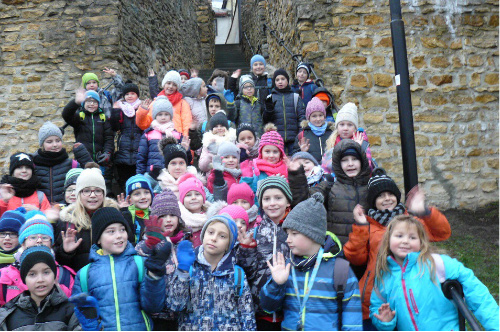
\includegraphics[width=1.5in]{zamek.jpg},{}] V pátek 7. prosince se žáci 1. – 4. třídy vypravili na zámek do Přerova. Krásná vánoční výzdoba zámku nadchla snad každého, stejně jako vyřezávaný betlém pana Zbořila, u kterého se hezky povídalo nejen o narození Ježíška. Děti si mohly také prohlédnout historické hračky a stavebnice. Nejvíce je zaujala dnes už legendární dánská stavebnice LEGO, která snad nechybí v žádném dětském pokojíčku. Adventní program na zámku ukončila výtvarná dílnička, ve které si děti podle své fantazie zdobily skleněnou baňku. Náš malý výlet jsme zakončili prohlídkou přerovského vánočního stromu a drobnými nákupy, na které se děti těšily. Ale i to k Vánocům patří.
\end{window}
\closearticle

\headline{\it\huge Vánoční Jarmark}
\lettrine{L}{etos} se poprvé těsně před adventem otevřely dveře naší školy pro všechny návštěvníky Vánočního jarmarku. Čekalo na ně mnoho stánků s rukodělnými dárečky a dekoracemi, které vyráběly děti i paní učitelky již několik týdnů před jarmarkem. Pro každého byly otevřeny i tvořivé vánoční dílničky.

V tělocvičně proběhl sváteční program - pohádka, kterou pro návštěvníky nacvičili naši třeťáci, scénka připravená ruštináři ze 7. třídy, taneční vystoupení kroužku paní Pěnkavové a nechybělo ani hraní vánočních koled a malé vánoční zpívání. Punč voněl po celé budově školy z vánoční kavárny s domácími lahůdkami, které připravily maminky a babičky. Zájemci si mohli zakoupit i tradiční vánoční hvězdy a prohlédnout si výstavku vánočních stromečků vyrobených do soutěže \uv{O nejkrásnější vánoční stromeček}.

\begin{window}[2,r,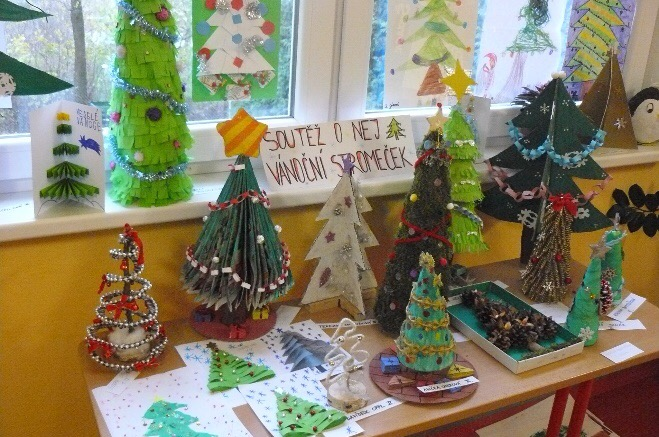
\includegraphics[width=2.3in]{soutez-stromek.jpg},{}] Akce trvala dvě hodiny, ale přesto za ní stojí spousta hodin práce všech, kteří se na její přípravě podíleli. Jim všem patří velké poděkování. Všem dětem, které vyráběly nebo prodávaly ve stáncích. Všem vystupujícím na vánočním programu. Všem rodičům i prarodičům, kteří pomohli vyrobit dekorace na prodej nebo pekli do kavárny. Všem učitelkám a učitelům naší školy, kteří celou akci organizovali. A samozřejmě i všem návštěvníkům, bez kterých by celá akce neměla smysl.
\end{window}

Věříme, že se první vánoční jarmark všem líbil a že se příští rok znovu uvidíme.
}\end{multicols}

\closearticle

\begin{multicols}{2}{
\byline{\it\Huge Čekám na signál}{Rostislav Lepař}

\lettrine{D}{oba} pokročila a technologie se neustále posouvají dál. Známe již 4G LTE  a zanedlouho tu jistě bude ve vzduchu 5G. A není to žádné sci-fi. Leč žijeme v kraji, kde máme jiné zkušenosti.

Určitě se mnohým z vás stalo, že lítáte po bytě, po dvorku a nehrajete žádnou dětskou hru, ale snažíte se jí dostat. Koho? Aspoň jednu čárku na displeji svého mobilního telefonu, abyste si mohli za nemalé peníze zavolat. Nebo již voláte, spojení se uskutečnilo, ale váš hovorový partner jen neustále opakuje, „špatně tě slyším", „ztrácíš se mi", „nerozumím ti". To nepopisuji rozchod po telefonu, ale nekvalitní spojení. Jednou z oblíbených hlášek je i „volaný nepřijímá, má buď vypnutý telefon nebo je mimo signál". Ano, možná se to někomu může zdát humorné, ale také jsou situace, kdy končí veškerá legrace. A to především tehdy, když potřebujeme, ať už z jakéhokoliv důvodu, kontaktovat integrovaný záchranný systém. Proč tenhle kolotoč? Protože operátoři dělají mrtvého brouka. Obrátili jsme se tedy na ně, aby nám situaci vysvětlili. Především v místních částech je tzv. signál hraničního dosahu vysílače a proto ty výkyvy v kvalitě pokrytí. A jejich rada? Co nejvíce nespokojených zákazníků, kteří se nebojí pro změnu něco malého učinit. 

Žádáme občany, aby prostřednictvím svého operátora poukázali, a to klidně i opakovaně, že nejsou spokojeni s kvalitou signálu. Nespokojenost a své poznatky ohledně kvality pokrytí mobilním signálem můžete psát i na obec. Chtěli bychom se s operátory domluvit na rozumném řešení a pokud by to bylo nutné, podílet se z rozpočtu obce na posílení těchto služeb nebo vybudování vhodného nového vysílače. Máme také zájem udělat průzkum, jakou účastnickou sílu mají jednotlivý operátoři a jaký je procentuální podíl našich občanů u jednotlivých operátorů. Změníme naši telekomunikační budoucnost? Spolu?
}\end{multicols}
\closearticle

\begin{multicols}{3}{
\byline{\sc\Large Obchůzka \uv{svatých Lucek} 13. 12. 2018}{Mgr. Ilona Sedláčková}

\lettrine{V}{rámci} celoročního projektu \uv{Rok s tradicemi} jsme dětem připomněli další starý lidový zvyk doby adventní, a to obchůzku \uv{Lucek}. Obcházení \uv{Lucek}, žen v bílých hábitech s ovázanými hlavami a čapími zobáky, je znám v našich krajích od 16. století. V předvečer svátku sv. Lucie chodily tyto \uv{Lucky} kontrolovat, zda mají hospodyně před Vánocemi uklizeno, neboť tyto bíle oděné ženy byly považovány za symbol čistoty.

Ve čtvrtek 13. prosince se to ve škole hemžilo bílými postavami s husími peroutkami a pomoučenými obličeji. Na tradiční obchůzku, která proběhla v dopoledních hodinách, se připravily čtyři žákyně ze čtvrté třídy. S rachotem se přiřítily do každé místnosti. Nejdříve ve společně zarecitované básni osvětlily přítomným podstatu starobylého obyčeje a poté se rozběhly po třídě, aby se vyptaly dětí, zda pomáhají s předvánočním úklidem, udržují pořádek, poslouchají, … Než děti stačily zareagovat, Lucky jim pohrozily a pomoučily je na tváře a po vlasech. Lucčinu znamení se nevyhnuly ani přítomné učitelky a asistentky. Nejvíce překvapeni byli tradičně prvňáčci. 

\begin{window}[2,r,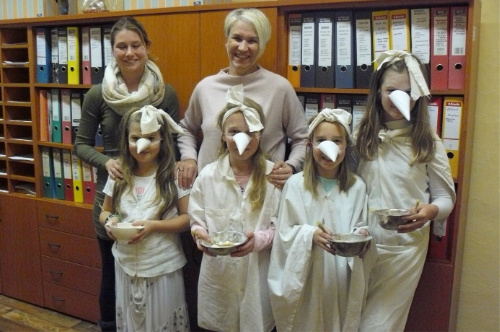
\includegraphics[width=2.3in]{lucky1.jpg},{}] Program pochůzky se následně opakoval ve druhé a třetí třídě a v některých třídách 2. stupně. Řádění Lucek si užily i děti v MŠ, kuchařky ve školní jídelně, paní ředitelka a další, kteří na Lucky narazili. 
\end{window}

\begin{window}[2,r,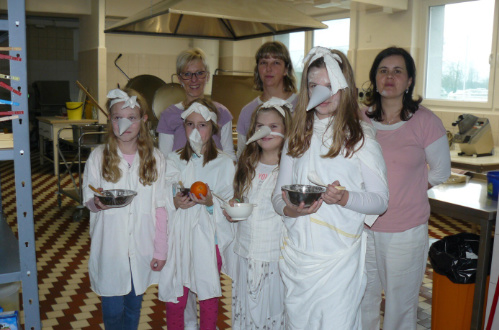
\includegraphics[width=2.3in]{lucky2.jpg},{}] Všichni byli spokojeni. Čtvrťačky si netradiční akcí nahradily tradiční výuku češtiny a matematiky, a zároveň ostatním přinesly trochu zábavy a poučení. 
\end{window}

\byline{\sc\Large Fyzikální workshop v Olomouci na Přírodovědecké fakultě}{Ľubica Havelková}

\lettrine{V}{předvánoční} době, 20.12. 2018, pozvala katedra fyziky žáky škol, kteří se účastní projektu PŘÍRODA na fyzikální pracovní dílny. Měli jsme tudíž tu možnost zúčastnit se různých zajímavých pokusů, které pro nás připravili studenti Přírodovědecké fakulty Univerzity Palackého v Olomouci.

\begin{window}[2,r,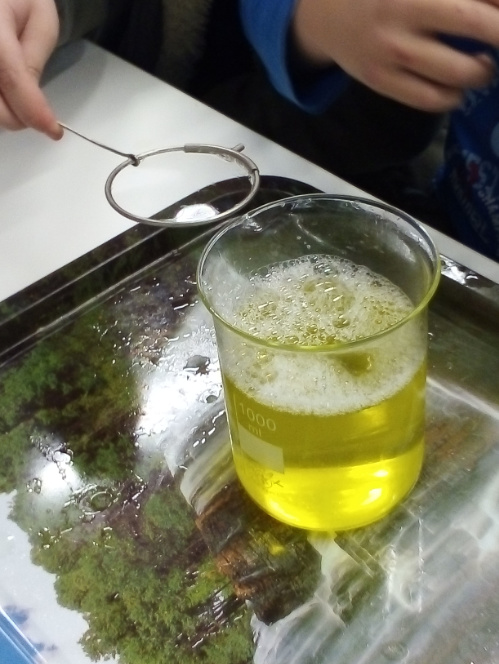
\includegraphics[width=1.5in]{fyzika.jpg},{}] Podle přiložených fotografií poznáte, s jakým zaujetím se 11 osmáků a 7 sedmáků věnovalo činnostem spojených s bádáním, které v běžném vyučování nemají možnost provozovat. Po třech hodinách vzrušujícího poznávání odcházeli žáci domů s různými nápady, které byli rozhodnuti realizovat jak doma, tak i ve škole. A že se jim to nakonec povedlo, můžou potvrdit i někteří učitelé, které ke svým pokusům pozvali. 
\end{window}
}\end{multicols}

\closearticle

\begin{multicols}{2}{
\byline{\sc\Large Zajímavosti z našeho kostela}{Anna Bilíková}

\lettrine{V}{roce} 1933 byl vymalován kostel nákladem 86 000 Kč. Manželé Antonín a Marie Bémovi č.p. 11 z Tršic, darovali na malbu 40 000 Kč. Ostatní peníze se získali sbírkami v kostele a přifařených obcích. Kostel byl malovaný od 11. 6. do 11. 10. 1933. Lešení pro malbu postavil podnikatel ve stavebnictví Antonín Grégr. Malbu provedl Jan Köhler, akademický malíř ze Stražovic u Kyjova. Jeho pomocníky byli: Jan Ježek, malíř z Bystřice pod Hostýnem a Antonín Skácel, pozlacovač z Přerova. Předsedou kostelního výboru byl Jaroslav Bém – rolník. Malba byla krásně provedena v moderním stylu a dodala lesk této krásné architektuře.

V roce 1990-1994 jsme se pustili do obnovy malby. Hlavním organizátorem této akce byl pan RNDr. Karel Březina, pan učitel Antonín Novák a paní učitelka Marie Najmanová. Do díla se zapojili i další farníci, kteří již nejsou mezi námi. 
Všem, kteří se zapojili, upřímné Pán Bůh zaplať. V dnešní době bychom to již nedokázali.
Snažili jsme se, pokud to šlo, malbu obnovit. Kdo přijde do tršického kostela, je ohromen jeho architekturou, krásou a výzdobou.
\closearticle

\byline{\sc\Large Jak jsme prožili vánoce v tršickém kostele Narození Panny Marie}{Anna Bilíková}

\lettrine{D}{oba} vánoční začíná adventem, to je čtyři týdny před Štědrým dnem, svěcením adventních věnečků. Je jich vždy přes 10 a je na co se podívat.  Rozsvěcujeme první adventní svíci.

Farníci nosí na první adventní neděli adventním věnečky k žehnání, rozsvěcuje se první svíčka. Je to obřad první adventní neděle. Od této doby za čtyři týdny je Štědrý den. Letošní rok vyšel Štědrý den na pondělí. Na Štědrý den již tradičně nám skauti dovezou betlémské světlo, a kdo má zájem, přijde k našemu kostelíčku se svíčkou a odnese si ho domů. Vzájemně si popřejeme, někdo ještě zajde na hřbitov a po setmění se i obec vylidní. Hospodyňky připravují štědrovečerní večeři a rodina se připravuje na štědrý večer. Ve 22:00 hod. jsme slavili mši sv. tzv. půlnoční. Tuto mši sv. sloužil P. František Foltýn. Na první svátek vánoční otevíráme kostel a rodiče přicházejí s dětmi k Betlému.

Pomalu se blíží svátek Tří králů. Je to úžasná akce snad pro všechny koledníky, organizátory i občany. Letos se vybralo v Tršicích a okolí 44 827 Kč. V Lipňanech se vybralo 3 406 Kč, na Zákřově 5 000 Kč, ve Vacanovicích 3 444 Kč, v Přestavlkách 4 010 Kč, v Hostkovicích 3 710 Kč, v Tršicích 20 974 Kč, v Lazničkách 4 283 Kč. Děkujeme všem štědrým dárcům.
}\end{multicols}

\newpage
\pagestyle{myinfo}

AAA

\end{document}
